\chapter{共享风险链路组分离路径算法研究}

\section{问题描述}
SRLG分离路径在它们之间没有任何共同的风险资源,也就是说,由于风险而导致的路径失败不会影响其他路径。图.\ref{fig:CompositeGraph}(b)显示两条SRLG分离路径对,表示为AP 和BP. 因为这两条路没有共同的风险资源,如果AP失败,BP仍然可以工作。本章主要讨论了两条不相交的路径保护路径,即可以描述如下。

\textbf{Min-Min SRLG分离路径问题}。给定一个图$G(V,E)$,每条链路$e_i\in \mathbb{E}$ 相关联一个权重权重$w_{e_i}$,一个源节点$s$和一个终结点$d$,找到一对$s$到$d$ 的SRLG分离路径对(表示为AP和BP),而且要求这两条分离路径中路径权重较小的那条路径权重最小化,形式如下:

\begin{equation}
\begin{array}{*{20}{c}}
   {\mathop {minimize}\limits_{AP,BP} } & {\min \left( {{w_{AP}},{w_{BP}}} \right)}  \\
   {subject\ to} & {{r_{AP}} \cap {r_{BP}}{\rm{ = }}\phi }  \\
   {} & {\mathbb{AP} \cap \mathbb{BP}{\rm{ = }}\phi }  \\
\end{array}
\label{eq:problem definition}
\end{equation}

即${w_{AP}}$ 和 ${w_{BP}}$是AP和BP的路径权重,$\mathbb{AP}$ 和 $\mathbb{BP}$分别是路径AP和BP上的链路集,${r_{AP}}$ 和 ${r_{BP}}$分别是影响路径AP和BP的SRLG集。


\begin{figure*}[tp]
  \centering
  % Requires \usepackage{graphicx}
  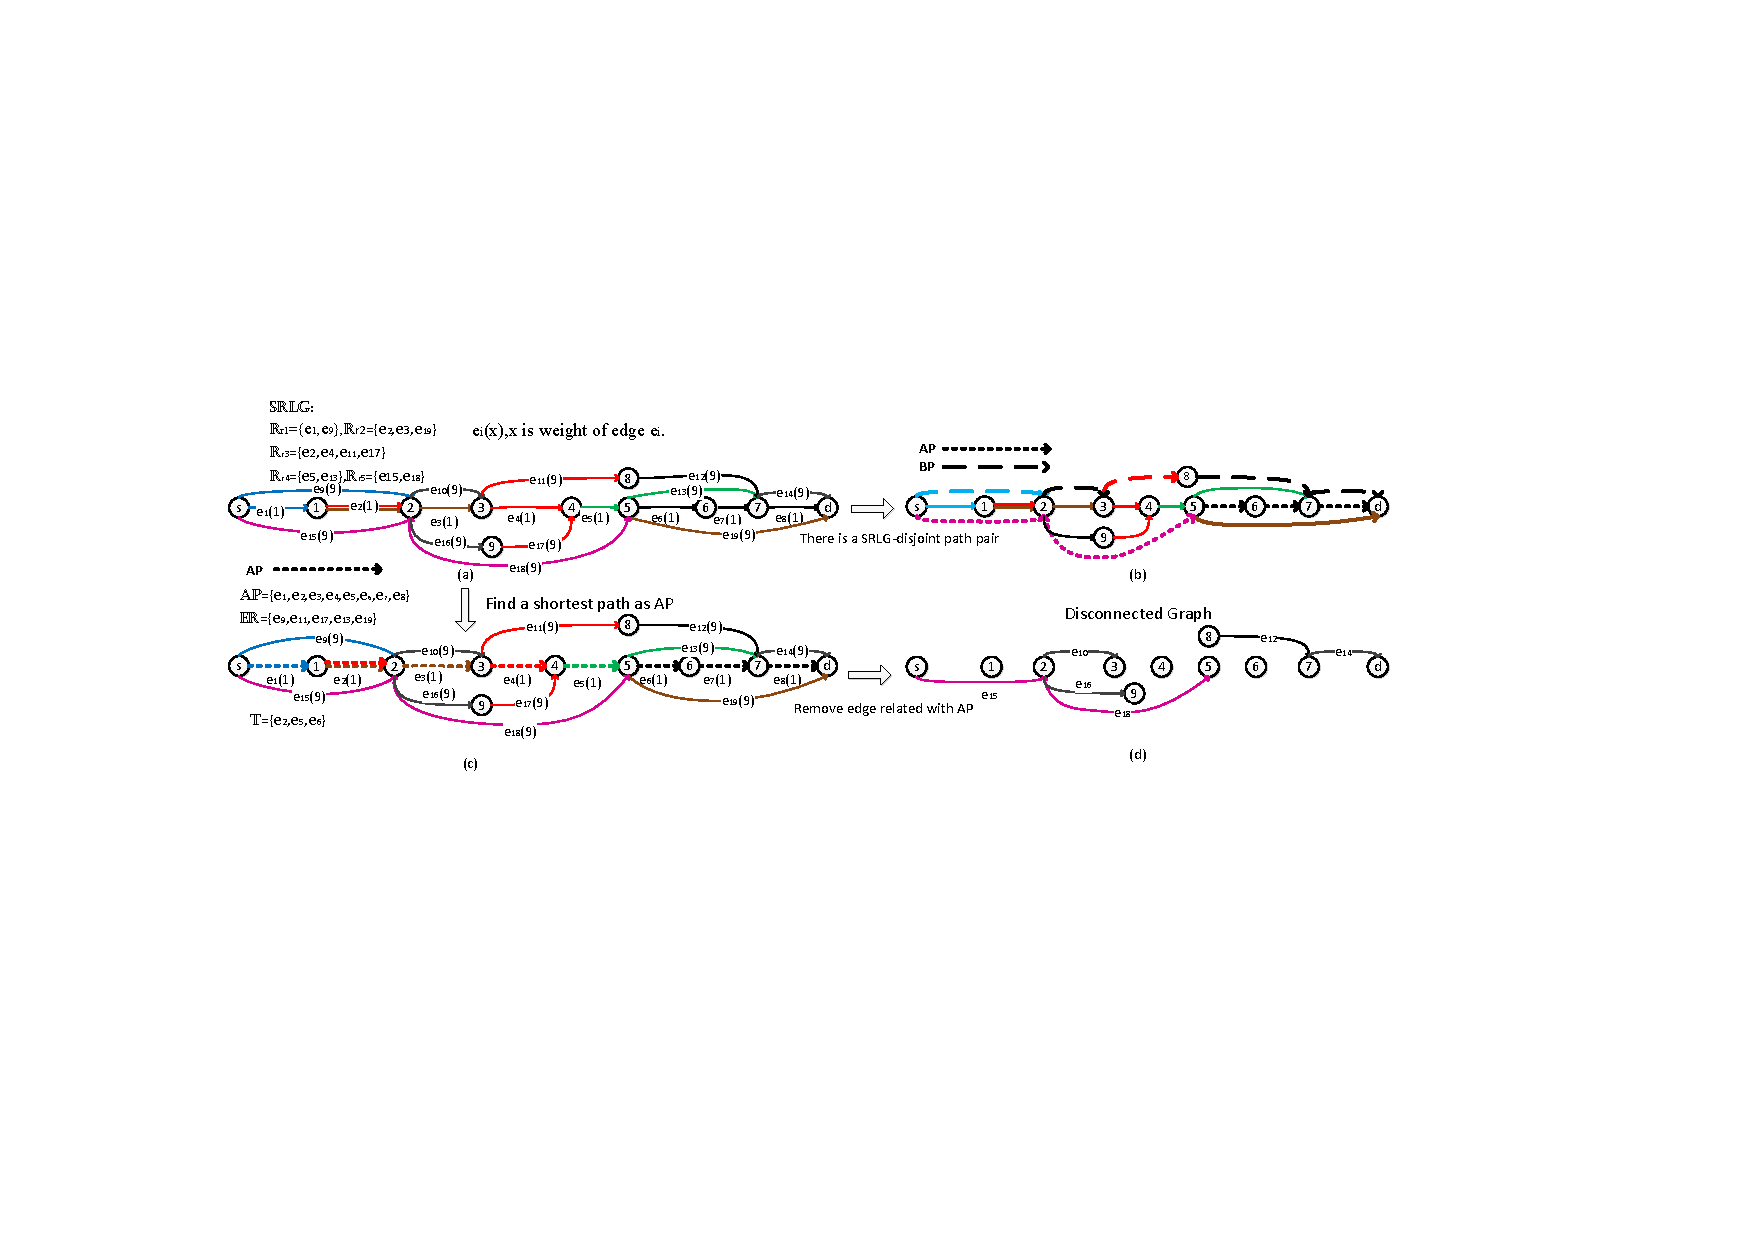
\includegraphics[width=7.2in]{figures/CompositeGraph}
  \caption{(a) A graph with five SRLGs: $\mathbb{R}_{r_1}=\{e_1,e_9\}$,$\mathbb{R}_{r_2}=\{e_2,e_3,e_{19}\}$,$\mathbb{R}_{r_3}=\{e_2,e_4,e_{11},e_{17}\}$,$\mathbb{R}_{r_4}=\{e_5,e_{13}\}$,$\mathbb{R}_{r_5}=\{e_{15},e_{18}\}$. (b)AP and BP in the graph. (c) The shortest weight path AP in the graph. $\mathbb{AP}=\{e_1,e_2,e_3,e_4,e_5,e_6,e_7,e_8\}$, $\mathbb{\mathbb{ER}}=\{e_9,e_{11},e_{17},e_{13},e_{19}\}$. (d)  Graph after deleting the links in $\mathbb{AP}$ and ${\mathbb{ER}}$. }
  \label{fig:CompositeGraph}
\end{figure*}

\section{原有算法概述}
共享风险链接组(SRLG)是一组链路共享相同的一个组件,该组件的故障会导致在这个组里所有链接的发生故障。就路径保护而言,尽管某些链路或者节点分离路径算法\cite{suurballe1984quick,bhandari1997optimal,li1990complexity,guo2003link,xu2004finding,beshir2011variants,guo2013finding,hu2003diverse} 已经提出来,SRLG分离路径 问题是比较棘手的,而且这些原有研究是限制在一定领域的。比如当每个SRLG只包含一条链路时,这个SRLG分离路由问题可以简化为链路分离路径问题,而通过节点分离方法(node split method)\cite{ford2015flows}节点分离路径问题可以转化为链路分离路径问题。因为SRLG组通常包括的链路超过一条并且网络中的链路通常可以属于多个SRLG组里,以至于求一对SRLG 分离路径问题比求一对链路或者节点分离路径问题要困难得多。

为了解决SRLG分离路径问题,一种可能的方法是0-1整数线性规划(ILP)\cite{hu2003diverse},通过分支限界法(branch-and-bound)来搜索来选择最优的主路径和备份路径。该方法时间复杂度高,不适用于大型网络。为了降低算法的复杂度,基于APF的启发式算法\cite{oki2002disjoint,li2002fiber,eppstein1998finding}能够求Min-Min SRLG分离路径问题的近似最优解。首先使用Dijkstra算法(或任何其他最短路径算法)求出主路径,求主路径时不考虑其相应的备用路径情况,在删除AP沿线的链路并且与AP共风险的节点和链路后,再利用最短路算法求的备用路径。

然而,使用APF启发式算法的有一个主要缺陷,一旦求得路径AP后也可能无法找到相对的SRLG分离路径BP,即使网络中确实存在一对分离路径。这就是所谓的“陷阱”问题,即使稠密网络中\cite{laborczi2001solving}这也是可能发生,在一个稀疏连接的网络中当然不能被忽略。陷阱有两种:不可避免的陷阱和可避免的陷阱。不可避免的陷阱是受拓扑约束的,任何算法都无法解决。如果网络不是2-边连通度的,则没有算法可以保证在拓扑中存在两个SRLG分离路径。另一方面,当两个节点之间存在SRLG分离路径对,但由于路由算法的缺陷而找不到时,就会出现一个可避免的陷阱。在本章中只考虑了可避免的陷阱。

对简单的APF算法的扩展,提出了KSP(K-最短路径)算法来处理节点/链路分离路径的陷阱问题。虽然它是处理陷阱问题最有效的算法之一,但它在大型网络中的性能受到影响,因为KSP 可能会涉及多路径搜索测试(K测试),直到它找到分离路径。当前候选的路径AP遇到陷阱问题后,仅根据路径长度选择下一个要测试的候选AP,而不考虑当前候选AP的那条链路(或那些链路)导致查找分离路径BP失败。因此,为了找到一对分离路径对,需要对大量的路径进行测试,这就引入了KSP算法中与K相关的时间复杂度。对于遇到陷阱问题的AP,我们应用从AP 路径导出的SRLG冲突链路集来指导将来的AP路径测试。这在很大程度上有助于减少寻找替代路径的时间复杂度。

其它SRLG分离路径算法\cite{rostami2012msdp,rostami2007cose,datta2008graph,xu2003new,todimala2004imsh},搜索最大SRLG分离路径对,并且路径间共享最小数目的公共链路。由于AP 和BP 可能具有相同的风险资源组,通过这种方法找到的解决方案是不可靠的。我们的算法目标是寻找完全SRLG分离路径。Xu\cite{xu2003trap}试图找到完全SRLG分离路径。但他的算法减少了问题的搜索空间,加快了路径搜索的速度。然而,它可能会以较大的代价返回路径,因为在削减后的空间可能会失去最优解。相反,为了大大加快搜索过程,我们利用SRLG冲突链接集将原问题划分为多个子问题,这些子问题可以并行执行。因此,我们的算法可以运行得更快,返回主路径成本非常低。

Datta\cite{datta2008graph}提出方法是将SRLG分离路径问题转化为链路分离路径问题,然后利用链路分离路径算法来解决。然而,只有特殊的SRLG模式(例如,星型)可以
将其转换为链路分离,这样就限制了该算法的广泛应用。当AP遇到陷阱问题时,CoSE\cite{rostami2007cose}算法试图找到一个SRLG集合,任何AP路径包含了这个SRLG集合里的所有SRLG,则必定找不到任何的与其对应的SRLG分离路径BP。CoSE 首先通过多轮搜索查找多个AP共享的SRLG,并且组成一个SRLG集合,然后根据SRLG集合来划分原始问题以搜索SRLG分离路径对。而不使用SRLG中链路之间共享风险的特性,CoSE方法的这种穷尽搜索需要非常高的计算开销。



\section{整数规划形式化}
\section{时间复杂度}
\begin{theorem}
\label{le:lemma1}
    Min-Min SRLG-分离路径问题是 NP-complete.
\end{theorem}
\begin{proof}
根据\cite{bhatia2006finding},Min-Min链路分离路径问题是NP-complete的。Min-Min链路分离路径问题是Min-Min SRLG-分离路径问题的子问题。设
Min-Min SRLG分离路径问题的复杂性为C(A),则NP-complete的$\leq$C(A).

为了求Min-Min SRLG分离路径问题的时间复杂度,我们首先假设了一个问题B(问题B的复杂性表示为C(B)),当找到两条的SRLG分离路径并且路径较小的路径其权重小于或等于M(M是大于零整数数)。Min-mim SRLG分离路径问题A与问题B等价,我们知道M必须大于零并且小于$\sum\limits_{e_i\in \mathbb{E}}w_{e_i}$。例如,我们假设0≤M≤10和m=6是最优解,通过经典的二分法(binary search method)时间复杂度为O(log(N)),如图.\ref{fig:binarySearch}所示,通过二分法我们得到了两条分离的路径,较小的路径其权重为m,因此问题A与 问题B等价。
\begin{figure}[tp]
  \centering
  % Requires \usepackage{graphicx}
  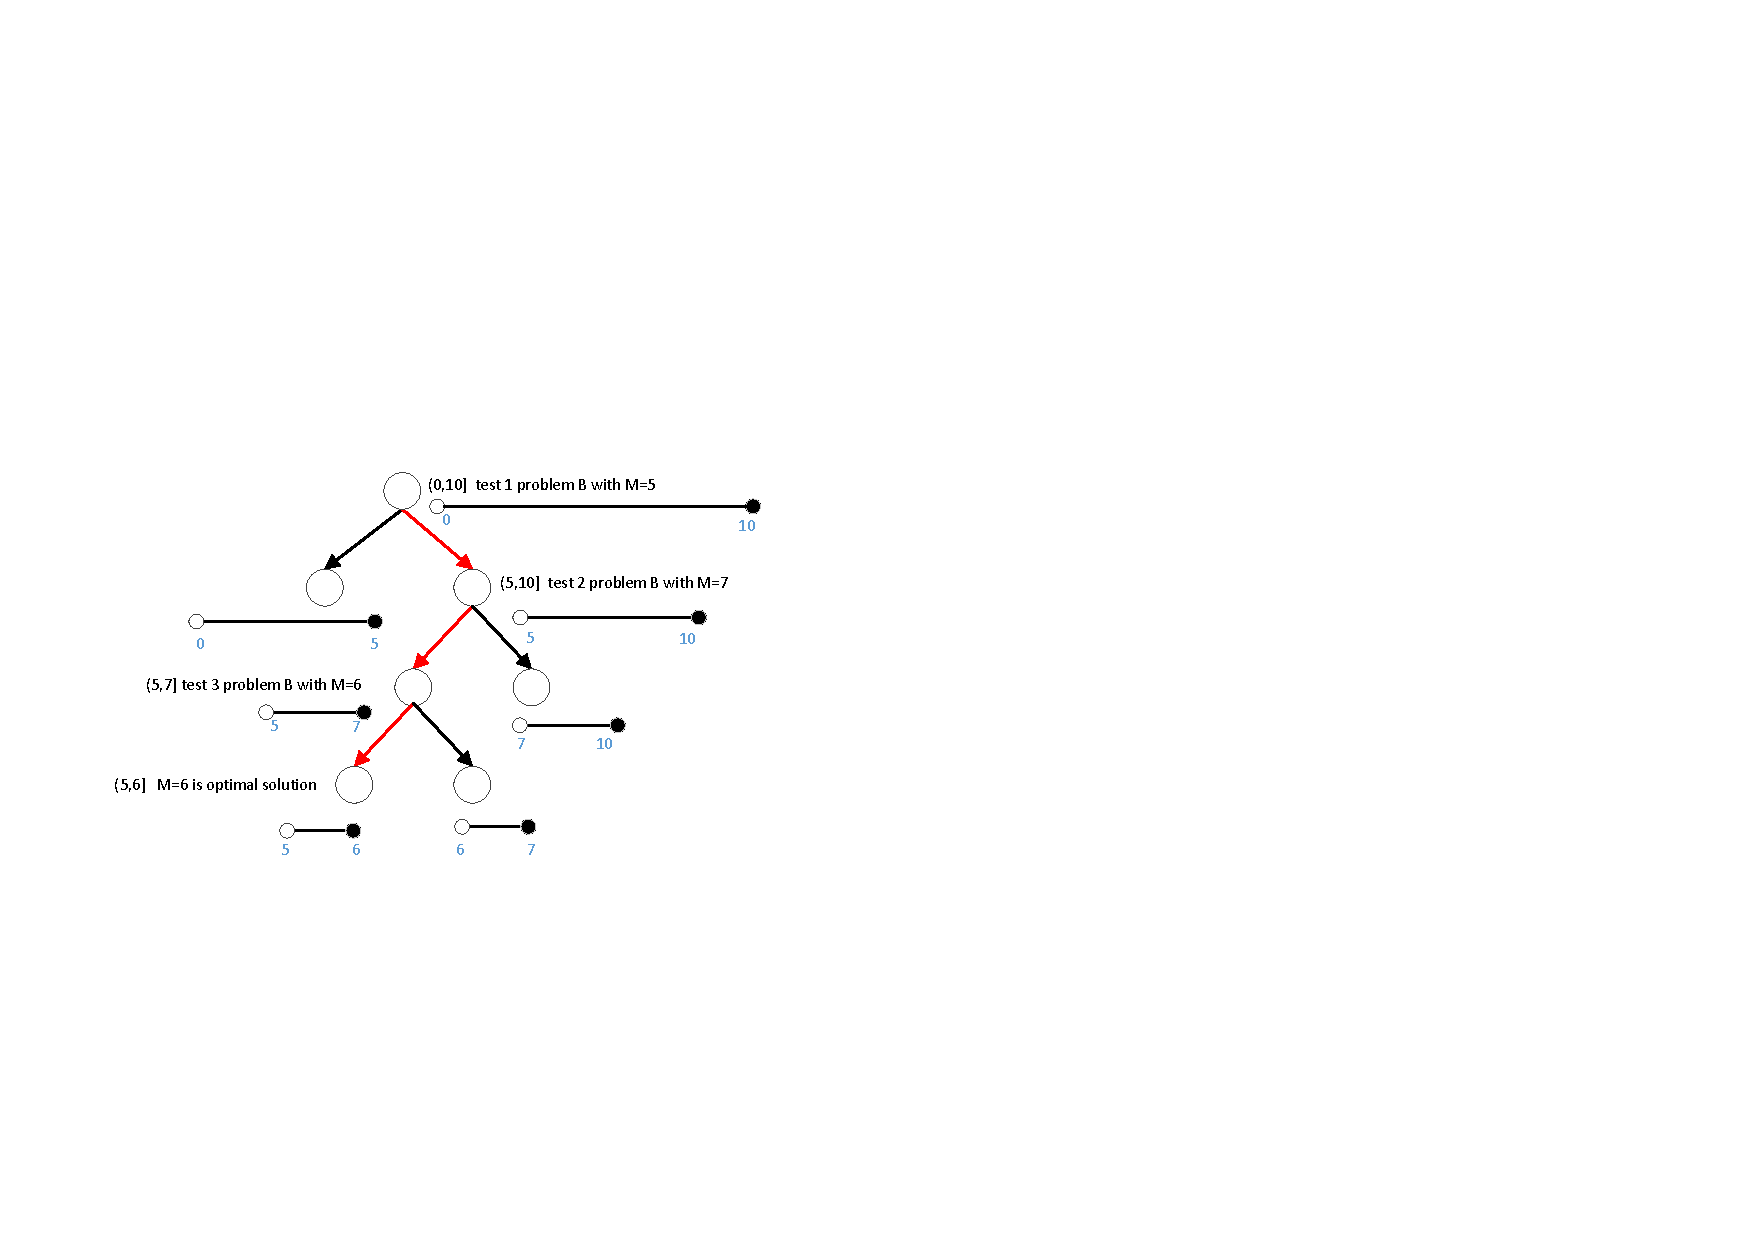
\includegraphics[width=3.0in]{figures/binarySearch}
  \caption{Request optimal solution M through Binary search method }
  \label{fig:binarySearch}
\end{figure}
假设程序X在输入问题B时,如果问题B没有解,则程序Y立即停止,否则程序B继续执行并获得问题B的解,因此问题B可以归结为NP-硬停止问题。因此C(B)$\leq$NP-hard。

此外,给定任意两条路径,很容易在多项式时间内判别这两条路径是否为SRLG分离路径,较小的路径其权重小于或等于M,从而使得C(B)$\leq$NP-complete。当B的复杂度等于A时,我们有C(A)=C(B)$\leq$NP-complete。因此,A=NP-complete。  
\end{proof}
\section{陷阱(trap)问题}
基于APF的启发式算法可能会陷入“陷阱”问题。也就是说,当一个AP被确定时,即使网络中确实存在一对分离路径对,它也可能无法找到SRLG分离的BP路径。图.\ref{fig:CompositeGraph}.(c),(d)说明了陷阱问题。虚线表示一个AP,其链路集为$\mathbb{AP}=\{e_1,e_2,e_3$ $,e_4,e_5,e_6,e_7,e_8\}$。在删除AP上的链路和与AP共享风险的链路后,图.\ref{fig:CompositeGraph}.(d) 所示的不存在从s到d的路径,因此找不到BP。

虽然KSP算法被认为是解决陷阱问题的有效算法,但它可能面临着效率低下的问题。在这个图.\ref{fig:KSPproblem}中,假设$e_1, e_2, e_3, e_4$的链路权重比其他链路大得多。此外,在$e_1, e_2, e_3, e_4$中,$e_1$ 和$e_2$的链接权重远小于$e_3$,$e_4$。然后,在KSP算法多次找从s到d的K短路时,总是包含$e_1,e_2$(虚线表示)。则最短AP 总会遇到陷阱问题,因为$e_1$和$e_4$ 具有相同的风险,因此无法找到BP。为了避免陷阱问题,必须将K设为一个大值,这给KSP带来了很高的时间复杂度。
\begin{figure}[htbp]
\centering
% Requires \usepackage{graphicx}
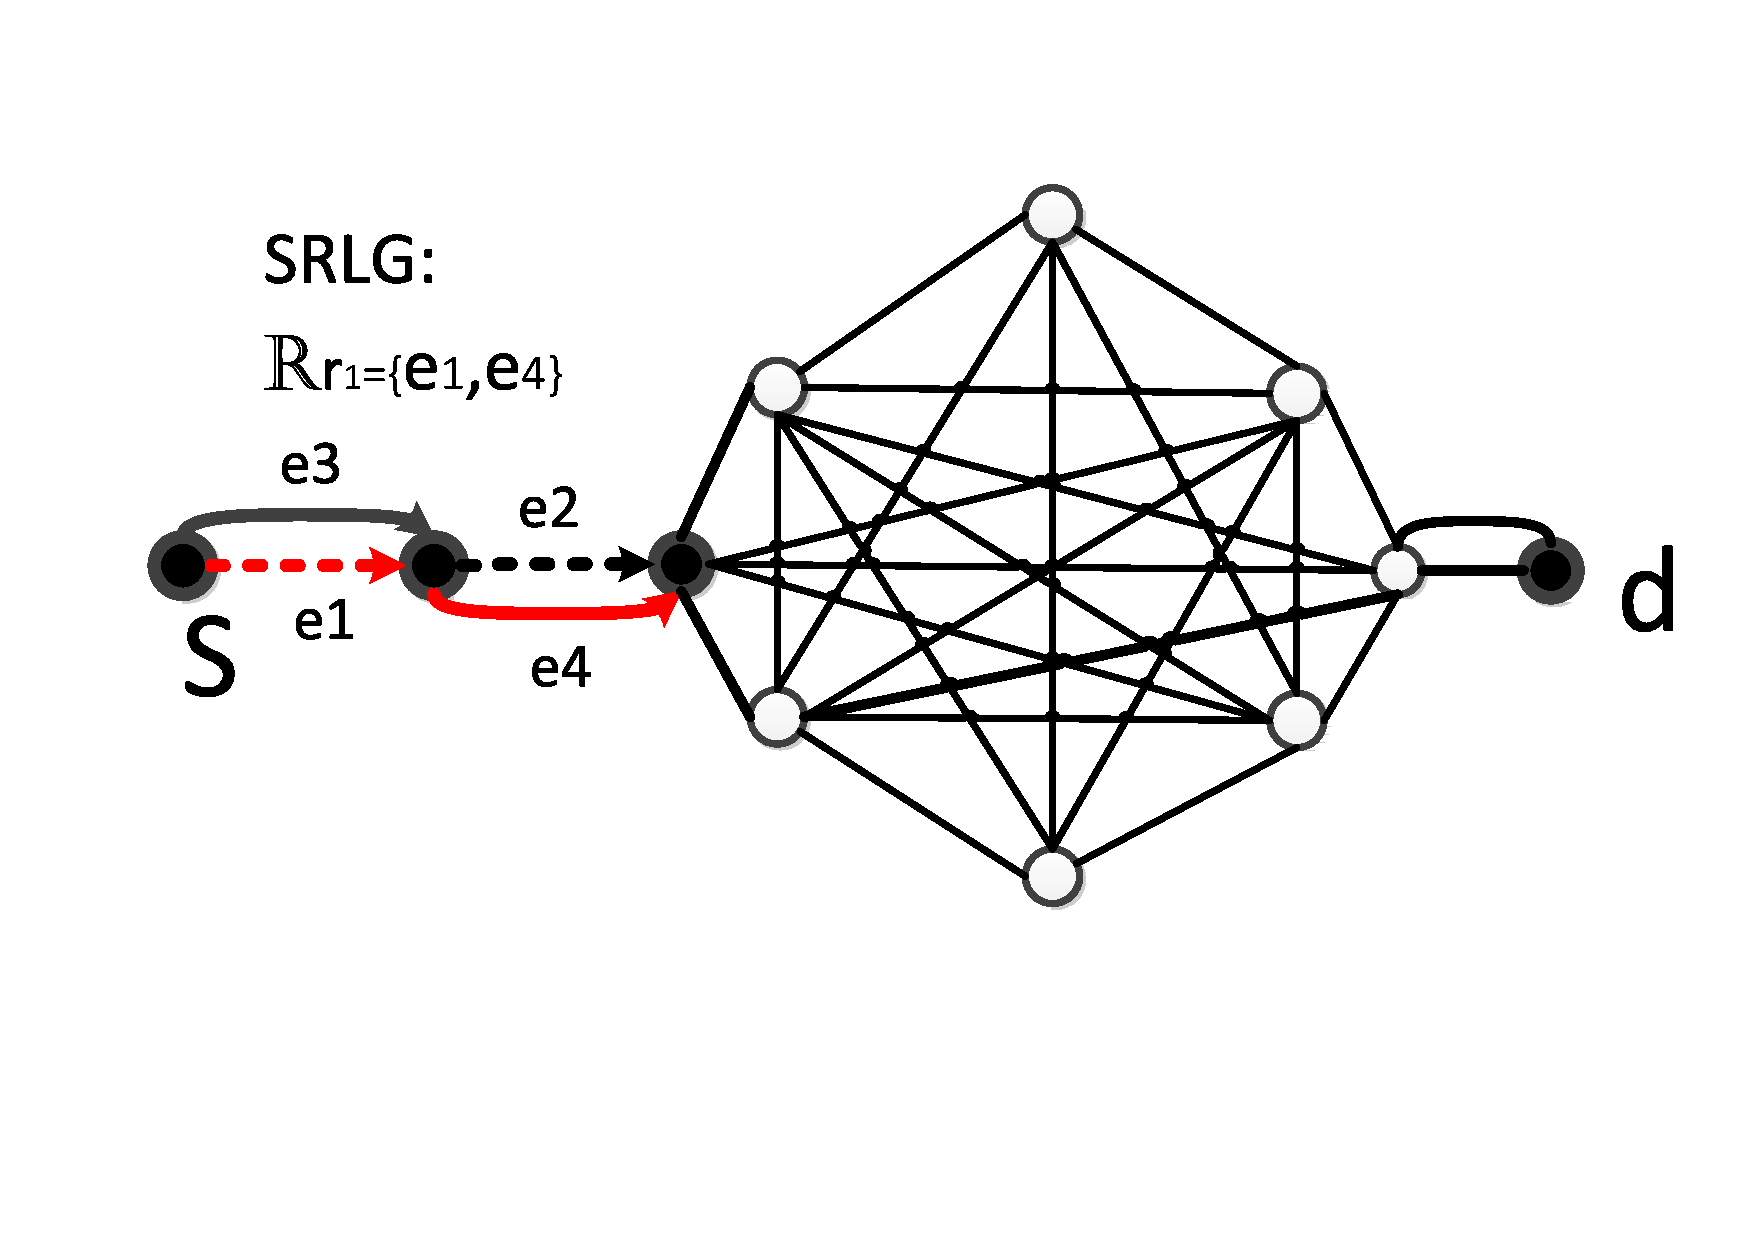
\includegraphics[width=2.8in]{figures/KSPproblem}
  \caption{An example to illustrate the inefficiency of KSP}
  \label{fig:KSPproblem}
\end{figure}


\section{分而治之的快速共享风险链路组分离路径算法}
当一个陷阱问题发生,并且对于给定的AP没有SRLG分离路径BP时,AP中可能存在一个子链路集,这样任何通过这个链路集里所有的这些“问题”链路的AP都不能找到一个SRLG分离BP。 我们称之为\textbf{SRLG冲突链路集}。与KSP不同,当最短AP遇到陷阱问题时,我们将通过两个主要步骤来解决这个问题。在图.\ref{fig:KSPproblem}的例子中,我们将首先找到图.\ref{fig:KSPproblem}中的SRLG冲突链路p集合,然后应用分而治之算法将原问题划分为两个子问题$\mathcal{P}(\emptyset,\{e_1\})$和 $\mathcal{P}(\{e_1\},\{e_2\})$。 这两个子问题可以在多核CPU平台上并行执行,快速得到SRLG分离路径对。
\subsection{分而治之}
在得到SRLG冲突链路集后,设计了一种分而治之的算法,将原Min-Min SRLG不相交路由问题划分为多个子问题,并行执行,加快了SRLG不相交路径对的查找过程。

为了便于问题划分,我们首先用I∩O=∅定义两个不相交的链接集I和O,其中我被称为包含集,O称为排除集。由P(i,O)表示的子问题(Min-Min SRLG-不相交问题),用于寻找一对AP和BP,其中AP是所有可能的AP中最短的,必须使用I中的链接,而不是O中的链接。

最初,让I=∅和O=∅,原来的Min-MinSRLG-不相交路由问题可以用P(∅,∅)表示.。注意,对于任何给定的链接,P(∅,∅)的解决方案(如果它存在的话)将使用包含或不包含链接的AP。给定SRLG冲突链路集T与E_1,e_2,···,e_T表示的T链路,原问题可按以下顺序划分。

除了子问题P({e1,e2,···,e T},∅)外,我们将试图为每个子问题找到一个最优解。
然后选择最好的路径对(即最短路径对)。
(AP)是原问题的最终(最优)解。
P(∅,∅)。如果这些子问题没有解决办法,
我们可以保证没有办法解决原来的
问题,因为我们划分问题的方式包括了所有的问题。
可能的路径。
就复杂性而言,解决问题所需的时间应该更少。
每个子问题至少比原来的问题本身
一个链接(来自T)将从任何进一步的
AP的路径计算,这也确保了不同的
AP将被发现,并测试是否存在一个SRLGdisnonovingBP。

当遇到陷阱问题时,我们的解决方案将原来的问题划分,并测试每个子问题以寻找最终的解决方案。在我们的分治解决方案中,子问题是基于从遇到陷阱问题的AP中发现的SRLG冲突链路集来测试的。与现有的算法相比,该算法在不考虑现有结果和问题的情况下,可以在很大程度上降低算法的计算量。对于图6中的例子,SRLG冲突链接集是T={e2,e5,e6}。分区过程如图6所示。根据SRLG冲突链路集,我们应该尝试总共3个标记子问题P({e2,e5},{e6}),P({e2},{e5})和P(∅,{e2}),其中选择AP路径权重最低的最优子问题P(∅,∅)作为最终的(最优)解决方案。注意,我们不需要解决子问题P({e2,e5},∅)和P({e2},∅),因为它们的解决方案已经包含在上面的子问题中。第一个解空间由两个子问题P({e2,e5,e6},∅)和P({e2,e5},{e6})组成。由于SRLG冲突链接集为T={e2,e5,e6},显然,子问题P({e2,e5,e6},∅)没有解决方案。因此,P({e2,e5},{e6})的解空间等于P({e2,e5},∅)的解空间。同样,P({e2},∅)的解空间包括P({e2}{e5},∅)和P({e2},{e5})的解空间。





\subsection{SRLG冲突链路集合}
\subsection{算法步骤}
\subsection{实验环境与评价指标}
\subsection{算法性能评估及比较}
